\documentclass[12pt]{article}
\setlength{\oddsidemargin}{0in}
\setlength{\evensidemargin}{0in}
\setlength{\textwidth}{6.5in}
\setlength{\parindent}{0in}
\setlength{\parskip}{\baselineskip}

\usepackage{amsmath,amsfonts,amssymb,bm,graphics,pgfplots,framed,dsfont,tikz,cancel}
\usetikzlibrary{decorations.markings}
\usepackage[scale=0.75,top=1cm,bottom=3cm]{geometry}

\begin{document}

\textbf{Minh Anh Nguyen }\\
\textbf{Discrete Mathematics\hfill Assignment 6}

\hrulefill

\begin{enumerate}
  \item Let $X = \{0,1,2,3,4\}$. Draw the graph associated with the $<$ relation on $X$. Should this graph be directed or undirected?
  \begin{center}
    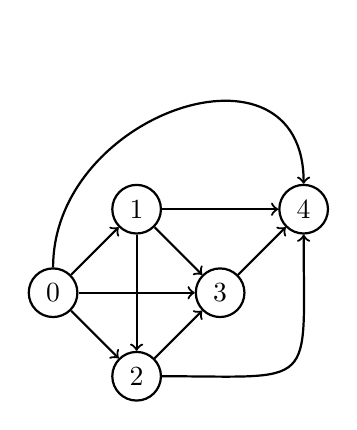
\begin{tikzpicture}[node distance={15mm}, thick, main/.style = {draw, circle}] 
        \node[main] (1) {$0$}; 
        \node[main] (2) [above right of=1] {$1$}; 
        \node[main] (3) [below right of=1] {$2$}; 
        \node[main] (4) [above right of=3] {$3$}; 
        \node[main] (5) [above right of=4] {$4$}; 
        \draw[->] (1) -- (2); 
        \draw[->] (1) -- (3); 
        \draw[->] (1) -- (4); 
        \draw[->] (1) to [out=90,in=90,looseness=1.5] (5); 
        \draw[->] (2) -- (3); 
        \draw[->] (2) -- (4); 
        \draw[->] (2) -- (5); 
        \draw[->] (3) -- (4); 
        \draw[->] (3) to [out=0, in=270,looseness=2] (5); 
        \draw[->] (4) -- (5); 
        \end{tikzpicture} 
  \end{center}
  textbfhe graph should be directed.
  \item Let $X = \{0, 1, 2, 3, 4\}$. Define a relation R on X such that $x R y$ if $x + y = 4$. Draw the graph associated with this relation. Should this graph be directed or undirected?
  \begin{center}
    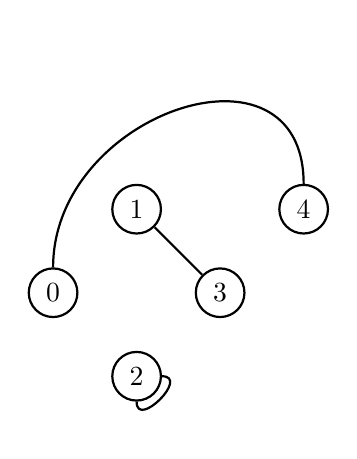
\begin{tikzpicture}[node distance={15mm}, thick, main/.style = {draw, circle}] 
        \node[main] (1) {$0$}; 
        \node[main] (2) [above right of=1] {$1$}; 
        \node[main] (3) [below right of=1] {$2$}; 
        \node[main] (4) [above right of=3] {$3$}; 
        \node[main] (5) [above right of=4] {$4$}; 
        \draw (1) to [out=90,in=90,looseness=1.5] (5);
        \draw (2) -- (4);
        \draw (3) to [out=0, in=270, looseness=2] (3);
        \end{tikzpicture} 
  \end{center}
  The graph should be undirected.
  \newpage
  For Exercises $3–6$, define a relation $\rightleftharpoons$ on the set S of all strings of letters: two strings are related if you can get one from the other by reversing one pair of adjacent letters. For example, $cow \rightleftharpoons ocw$ but $cow \text{~} \cancel{\rightleftharpoons} \text{~} woc$.
  \item Consider all the strings you can form with the letters c, a, and t (there are six). Draw the graph whose nodes are these six strings and whose edges represent the $\rightleftharpoons$ relation. Should this be a directed or an undirected graph?
  \begin{center}
    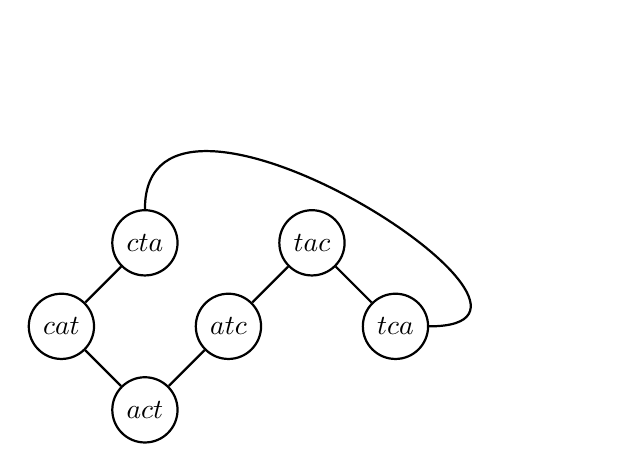
\begin{tikzpicture}[node distance={15mm}, thick, main/.style = {draw, circle}] 
        \node[main] (1) {$cat$}; 
        \node[main] (2) [above right of=1] {$cta$}; 
        \node[main] (3) [below right of=1] {$act$}; 
        \node[main] (4) [above right of=3] {$atc$}; 
        \node[main] (5) [above right of=4] {$tac$};
        \node[main] (6) [below right of=5] {$tca$}; 
        \draw(1) -- (3);
        \draw(1) -- (2);
        \draw(3) -- (4);
        \draw(4) -- (5);
        \draw(5) -- (6);
        \draw (2) to [out=90,in=0,looseness=1.5] (6);
        \end{tikzpicture} 
  \end{center}
  This should be an undirected graph.
  \item Find an Euler path in the graph you made in Exercise 3.\\
  The Euler path from the graph in Exercise 3 is: 
  \[cta \rightarrow cat \rightarrow act \rightarrow atc \rightarrow tac \rightarrow tca \rightarrow cta\]
  \item Consider the graph formed by the $\rightleftharpoons$ relation on the set of all the strings you can form from the letters l, y, n, and x. Does this graph have an Euler path? Why or why not?\\
  From the letters l, y, n and x, I can construct 24 strings. Each of those will have 3 possibilities to form a new string by reversing a pair of adjacent letters. \\
  Hence, each of the 24 vertices had an odd degree of 3 edges.\\
  Therefore, the graph does not have a Euler Path.
  \item Does the graph of the $\rightleftharpoons$ relation on the set of all strings formed from the letters l, e, o, p, a, r, and d have an Euler path? Why or why not?\\
  The number of string we can construct from the letters l, e, o, p, a, r and d is 5040 strings. Each of them has 6 possibilities to form a new string.\\
  Hence, the graph does have a Euler Path since they only have an even degree of 6 edges.
  \item Suppose you wanted to model an equivalence relation with a graph. Would you use a directed or an undirected graph? What would the equivalence classes look like? Explain.
  
\end{enumerate}
\end{document}